%!TEX root=../ast2016.tex

\vspace{-.5em}

\section{Experimental Setup}
\label{sec:experimental-setup}

% PURPOSE: Give the lead in to the research questions and then formally state each question

To experimentally evaluate the presented \vma technique, we investigate three research questions, comparing it against
the \Original approach to mutation analysis for relational database schemas, which uses an actual instance of a DBMS
(and is hereafter simply referred to as the ``\Original'' method).

% PSM changed the colon to a full stop because the next part currently starts on a new column and it looked odd

\vspace{5pt}

\noindent
\textbf{RQ1 (Efficiency):} How does the time overhead of \vma compare to the \Standard technique's cost, and how does
this vary depending on the DBMS in use?

\vspace{5pt}

\noindent
\textbf{RQ2 (Time Savings):} How does the time savings from using \vma vary when increasing either the number
of analysed mutants or the number of executed tests?

\vspace{5pt}

\noindent
\textbf{RQ3 (Effectiveness):} How does the mutation score of \vma compare to the score of a time-constrained \Original method that
is only permitted to run for as long as the virtual one?

% PURPOSE: Explain the number of trials and the basics about test data generation and describe the subject schemas,
% making sure to briefly mention that the chosen DBMSs are representative in nature (could not fit more content)

% {Schema} & \HyperSQL & \Postgres & \SQLite \\
% JWhoisServer & 178 & 178 & 184\\

\begin{sloppypar}
\inlineheading{Methodology} To answer the first and second research \mbox{questions}, we recorded the time needed to run the \Original approach and \vma 30 times each, for each of the subject schemas listed in Table~\ref{tbl:study-schemas} and with each of the three representative DBMSs --- \HyperSQL, \Postgres and \SQLite.  Two schemas we used appear in open-source projects (i.e., JWhoisServer and MozillaPermissions), while others appear in SQL conformance suites and DBMS sample sets (i.e., NistWeather and Iso3166, respectively). Previous studies have shown that the remaining schemas were challenging to handle for random test generators \cite{McMinn2015} and the open-source DBMonster tool \cite{Kapfhammer2013}.  Between $9$ and $184$ mutants were generated for each schema and between $426$ and $449$ in total for the three DBMSs. These totals correspond to numbers following the removal of certain ineffective mutants --- mutants found to be equivalent to the original or some other mutant, or ``stillborn'' \cite{Wright2014}. Due to differing interpretations of the SQL standard, the notion of ``equivalence'' differs from DBMS to DBMS, leading to a different number of mutants for some of the schemas (e.g., JWhoisServer yields $178$ for \HyperSQL and \Postgres and $184$ for \SQLite).
\end{sloppypar}

% PURPOSE: Give more details about the test data generation procedure

For each run, we used a test suite that was automatically generated by a search-based method with a unique random seed.  Details of the specific generation algorithms used are given by McMinn \etal~\cite{McMinn2015}. We used the alternating variable method, or \AVM, since past experiments have show it to be the most reliable automated method for generating test suites that achieve high levels of test coverage~\cite{McMinn2015}. The coverage criterion we used was a combination of ``ClauseAICC'', ``AUCC'' and ``ANCC'', thus merging the strongest criteria for testing the integrity constraints of schemas.

% PURPOSE: Explain the third research question's process

To answer the third research question, we ran the \Original technique $30$ times, performing a mutation analysis that randomly selected mutants until the time taken for the corresponding run of the $30$ repetitions of \vma was exhausted. In other words, the \Original method was run in a ``time-constrained'' fashion where its maximum allotted time was equal to the time needed to complete the comparable \vma.

% PURPOSE: State the execution environment and the tools used for the experiments

We implemented our virtual model into our \SA tool \cite{Kapfhammer2013,McMinn2015,Wright2014}, which we also used to
perform all of the experiments. \SA was compiled with the JDK 7 compiler and executed with the Linux version of the 64-bit Oracle Java 1.7 virtual machine.  Experiments were executed on an Ubuntu 14.04 workstation, with a 3.13.0-44 Linux 64-bit kernel, a quad-core 2.4GHz CPU and 12GB RAM. All input (i.e., the database schemas) and output (i.e., the result files) were stored on the workstation's local disk. We used the default configuration of \PostgreSQL version 9.3.5, \HyperSQL version 2.2.8 and \SQLite 3.8.2.  \HyperSQL and \SQLite were used with ``in-memory'' mode enabled.

% PURPOSE: Describe the meaning of the box and whisker plots

\inlineheading{Analysis Methods} Figures~\ref{fig:graphic_bwplot_schema_analysistime_org_vm} and ~\ref{fig:graphic_bwplot_schema_mutationscore_vm_tcm} furnish box and \mbox{whisker plots}.  In these plots the box itself represents the interquartile range (IQR), or the measure of statistical dispersion that is the difference between the first and third quartiles. Moreover, the upper whisker extends from the top of the box to the highest value that is within $1.5$ times the IQR, the lower whisker goes from the bottom of the box to the lowest value within $1.5$ times the IQR, and the thick horizontal line represents the median value. Also, these box plots use a filled circle for an outlier and an open diamond for the mean value.

% PURPOSE: Describe the statistical and effect size tests

To statistically analyse the trends in Figure~\ref{fig:graphic_bwplot_schema_analysistime_org_vm} we conducted tests for significance with the nonparametric \wilcoxon, using the sets of 30 execution times obtained with a specific DBMS and the \Original and \vma techniques.  A \pvalue less than $0.05$ is deemed to be significant.  To complement significance tests, the nonparametric \^{A}\textsubscript{12} statistic of Vargha and Delaney \cite{Vargha2000} was used to compute effect sizes, which determine the average probability that one approach ``out performs'' another.  We followed the guidelines of Vargha and Delaney in that an effect size is deemed to be ``large'' if the value of \atwelve~is $< 0.29$ or $> 0.71$, ``medium'' if \atwelve~is $< 0.36$ or $> 0.64$ and ``small'' if \atwelve~is $< 0.44$ or $> 0.56$.  Values of \atwelve~close to the $0.5$ value are viewed as showing no effect.  When discussing effect sizes for the execution times of the two methods, we follow Neumann \etal~\cite{Neumann2015} and say that a value of \atwelve closer to zero indicates that virtual is the preferred technique while a value near one shows that \Original is faster.

% PURPOSE: Describe the calculation of the percentage of mean time saved

As the number of mutants subject to analysis and the number of generated tests increases, Figure~\ref{fig:graphic_scatterplot_mutantstests_percentagetimesaved} plots the percentage of mean time saved from using \vma instead of the \Original method.  This value is determined by first calculating the mean execution time from the thirty trials of both the \Standard and the \virtual techniques. If $T_s$ denotes the mean time taken by the standard method and $T_v$ is the mean time needed for the virtual one, then we calculated the percentage of mean time saved by $({T_s - T_v})/{T_s}$.

% PURPOSE: Describe the calculation of the correlation coefficient

We employed a correlation statistic to determine how the mutation scores of the \tc method correspond to those of \vma.  Due to the possibility of rank ties, which are not supported by a number of correlation measures, we chose to use the tie-aware Kendall's \taub~coefficient, as provided by the ``Kendall'' R package \cite{KendallCran}.  Kendall's \taub~provides a measurement of correlation between -1 and 1, representing a strong negative and strong positive association, respectively, with 0 indicating that there is no correlation. Following Inozemtseva and Holmes, we adopt the Guildford scale to describe the correlation values, with the absolute value of a coefficient being described as ``low'' when it is less than $0.4$, ``moderate'' when it is between $0.4$ and $0.7$, ``high'' when ranging from $0.7$ to $0.9$, and ``very high'' when it is greater than \mbox{$0.9$ \cite{Inozemtseva2014}}.

% GRAPHIC: This is the figure that will contain the graphs for the percentage and the number of mutants (and tests)
% NOTE: This input had to be moved to this location in the code to ensure that the graphs were properly spaced.
% SCATTERPLOT INPUT
%!TEX root=ast2016.tex

\begin{figure*}[t]
  \centering
  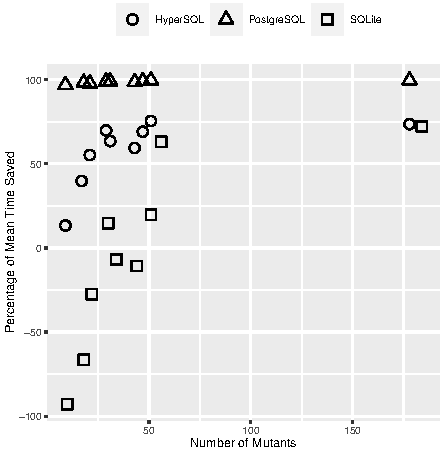
\includegraphics[scale=1.0]{graphics/graphic_scatterplot_nummutants_percentage.pdf}
  \caption{Box plot of the execution time for the original and virtual mutation analysis techniques.}
  \label{fig:graphic_bwplot_schema_analysistime_org_vm}

  % Details about the box plot from the R documentation:

  % The lower and upper "hinges" correspond to the first and third quartiles (the 25th and 75th percentiles). This differs
  % slightly from the method used by the boxplot function, and may be apparent with small samples. See boxplot.stats for for
  % more information on how hinge positions are calculated for boxplot.

  % The upper whisker extends from the hinge to the highest value that is within 1.5 * IQR of the hinge, where IQR is the
  % inter-quartile range, or distance between the first and third quartiles. The lower whisker extends from the hinge to
  % the lowest value within 1.5 * IQR of the hinge. Data beyond the end of the whiskers are outliers and plotted as points
  % (as specified by Tukey).

  % Commentary on the results in this output:

  % - Note that this data has been "log transformed" using a log-to-the-base-ten transformation
  % - Transformation is done because the Postgres-Original data is on a different scale than all other data
  % - This means that you will only see variation for Postgres-Original (without transformation)
  % - Using the log-transformed data shows the basic trends in the data sets

  {\small \justifying{ \noindent In this plot the box itself represents the interquartile range (IQR), or the measure of
      statistical dispersion that is the difference between the first and third quartiles. Furthermore, the upper
      whisker extends from the top of the box to the highest value that is within 1.5 times the IQR, the lower whisker
      goes from the bottom of the box to the lowest value within 1.5 times the IQR, and the thick horizontal line
      represents the median value. The boxes in this plot are noticeably compressed because there is little variance in
      the timings across the different configurations.  Since the results from running the original method on the
      \Postgres DBMS differ substantially from those with the other techniques and databases, all of the
      data values were log-transformed, thereby best revealing the relevant trends.} \par}

\end{figure*}


% GRAPHIC: This is the box and whisker plot that shows the mutation score for the two techniques
% BOXPLOT input
%!TEX root=ast2016.tex

\begin{figure*}[t]
  \centering
  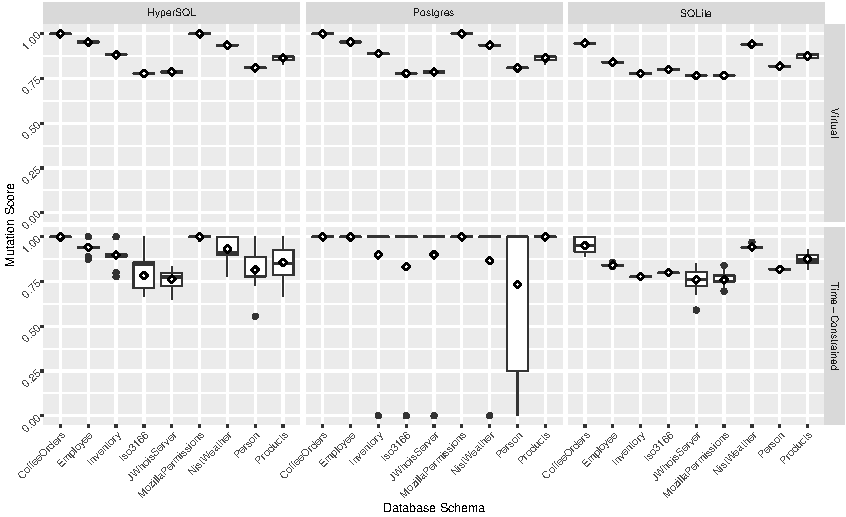
\includegraphics[scale=1.0]{graphics/graphic_bwplot_schema_mutationscore_vm_tcm.pdf}
  \caption{Box plot of the mutation score for the virtual and time-constrained mutation analysis techniques.}\label{fig:graphic_bwplot_schema_mutationscore_vm_tcm}

  % NOTE: This caption is not yet correct.

  {\small \justifying{\noindent The meaning for this box plot's elements is the same as the meaning of those described
      in the subcaption of Figure~\ref{fig:graphic_bwplot_schema_analysistime_org_vm}. Additionally, in this box plot a
      filled circle denotes an outlier and the open diamond is the mean value. Using test suites from thirty separate
      runs of the search-based test data generation method developed by McMinn \etal~\cite{McMinn2015}, this plot shows
      the variation in the mutation score for both the virtual and the time-constrained method and for all of the chosen
  relational schemas and the three database management systems. } \par}

\end{figure*}


% These are the threats to validity:

% -- Randomness in the SA tool and the generated test suite
% -- Randomness in the selection of mutants for time-constrained
% -- Variability in the running time of the mutation analysis
% ---> So, ran multiple trials and did statistical analysis
% ---> When calculated effect sizes, we also looked at thresholds

\inlineheading{Threats to Validity} There are several threats to the validity of the empirical results presented in this paper. First, several of the techniques that we used (e.g., the test data generator in \SA and the mutant selection by the \tcm~method) employ randomness. Additionally, background processes running during experimentation may introduce small random differences in the timings for the mutation analysis methods. To control for these threats we ran 30 trials and used box and whisker plots and statistical tests to analyse the results. Adhering to the advice of Neumann \etal~\cite{Neumann2015}, we disregarded all timings below $100$ ms --- as they would not be perceived by users of our tool --- to ensure that we did not misapply the Vargha-Delaney \mbox{effect size}.

% -- Defects in the test data generator
% -- Defects in the virtual mutation analysis
% ---> So, we tested these programs and checked the mutation scores

% -- Defects in the analysis routines
% --> So, we tested this these programs

Another threat to the validity of our results is defects in the test data generator or one of the mutation analysis techniques. We controlled these threats by implementing and regularly applying an automated test suite for all of these software tools; to ensure their correct operation we also manually performed ``spot checks'' on small schemas. In addition, we verified that the \vma always yielded the same mutation score as the \Original one. Finally, since defects in our analysis routines would compromise the conclusions from our experiments, we created and regularly ran tests for the R code that manipulated the data, performed statistical tests and effect size computations, and visualised the results.

% -- Limited number of subjects in the empirical study
% --> But, these subjects are "representative" and open-source

While the rich and diverse nature of real software systems makes it impossible for us to claim that our schemas are representative of all the characteristics of all possible relational database schemas, we endeavored to select schemas from a wide variety of sources, comprising open-source programs, conformance suites for the SQL standard and schemas from databases that were used in previous studies. Table~\ref{tbl:study-schemas} shows the variety captured by the schemas, with tables that contain 1--50 constraints, including \CHECKs, \FKs, \PKs, \NOTNULLs and \UNIQUEs.
